\documentclass[11pt]{article}

\usepackage[margin=1in]{geometry}
\usepackage[utf8]{inputenc}
\usepackage{hyperref}
\usepackage{graphicx}
\usepackage{booktabs}
\usepackage{amsmath}
\usepackage{amssymb}
\usepackage{xcolor}
\usepackage{natbib}
\usepackage{tikz}
\usetikzlibrary{arrows.meta, positioning, shapes.geometric}

\hypersetup{
  colorlinks=true,
  linkcolor=blue!50!black,
  citecolor=blue!50!black,
  urlcolor=blue!50!black
}

\title{Do Not Grade Your Own Homework: Externalized Verification Gates,
Evidence-Derived Hypothesis Trees, and Grounding-Based Confidence Capping
for LLM Root-Cause Agents}

\author{Victor Robin\\ BlueRobin (independent homelab research)}

\date{June 2026}

\begin{document}

\maketitle

\begin{abstract}
Large-language-model (LLM) agents that perform root-cause analysis (RCA) on
production incidents fail in characteristic, well-documented ways: they
self-validate conclusions that no tool ever supported, they terminate
prematurely on an ``I'm done'' assertion, and they report high confidence in
ungrounded hypotheses. This paper describes the reasoning-safety core of the
BlueRobin Debug Agent --- a .NET, human-in-the-loop RCA agent operating
against a self-hosted homelab at a $\sim$50~EUR/month budget --- and how its
design is driven directly by the MAST agentic-failure taxonomy
\citep{cemri2025mast}. We contribute three interlocking mechanisms. First, an
\emph{externalized deterministic verification-gate finite-state machine}
(\texttt{VerificationGate}) that lives outside the model and governs loop
termination, replacing \texttt{MaxTurns} as the sole stop; a ``confident''
exit \emph{requires} hard tool evidence, and ``no confident root cause'' is a
first-class outcome. Second, \emph{evidence-derived hypothesis state with
provenance} (\texttt{HypothesisModel}), in which each candidate's state in
$\{\textrm{Validated}, \textrm{Invalidated}, \textrm{Inconclusive}\}$ is
computed from real-tool evidence whose source is never \texttt{llm-inferred},
captured through an \texttt{EvidenceCapturingTool} decorator and a
negation-aware, structured-signal-first verdict classifier. Third, an
\emph{evidence-chain assembler} with a \emph{grounding-based confidence
soft-cap} ($\textrm{CapPartial}=0.84$, $\textrm{CapUngrounded}=0.64$) that
bounds the LLM's self-rated confidence below the action tiers (issue 0.40 /
patch 0.65 / PR 0.85), so an ungrounded conclusion can never reach the
pull-request tier. Nothing auto-remediates. We position this work honestly:
it is a systems and engineering-discipline contribution, not an empirical
breakthrough, and we discuss its threats to validity at length.
\end{abstract}

\section{Introduction}

A root-cause-analysis agent receives an alert (``Authelia OIDC returning 500s
after an LLDAP schema change'') and must localize the failing component,
explain why, and propose a fix. The naive approach --- hand the alert text to
a frontier model and ask for the root cause --- fails for a structural reason:
the model has no access to the live system, so it pattern-matches the alert
against its training distribution and emits a plausible-sounding hypothesis
with no grounding in the actual incident. The agentic correction is to give
the model tools (query traces, tail logs, read deploy history) and let it
reason--act--observe in a loop \citep[ReAct;][]{yao2022react}. But the agentic
loop introduces its \emph{own} failure modes.

The MAST taxonomy (Multi-Agent System Failure Taxonomy;
\citealp{cemri2025mast}), derived by IBM and Berkeley from 310 ITBench traces,
quantifies them: the dominant failures are \textbf{incorrect self-verification,
premature termination, memory loss, and reasoning-action mismatch}, together
accounting for roughly 94\% of observed failures. Translated into design
rules: \emph{never let the LLM grade its own homework}; \emph{require hard tool
evidence before exit}; \emph{enforce termination via a finite-state machine
outside the model}; and \emph{make ambiguity a first-class branch}. These are
not abstractions for us --- they are the literal contract comments in the
BlueRobin Debug Agent source.

The honest ceiling for autonomous RCA is low. The best agent on OpenRCA
\citep{xu2025openrca} reaches $\sim$11.3\% exact-match; the best frontier model
on IBM ITBench-AA \citep{itbenchaa2026} reaches $\sim$47\%
precision-at-full-recall. An advisory, human-in-the-loop posture is therefore
\emph{the state of the art}, not a concession. A human always merges in
BlueRobin; the agent's job is to produce a well-grounded, auditable hypothesis
and let the operator decide.

This paper's contributions are:
\begin{itemize}
  \item \textbf{An externalized verification-gate FSM}
  (\texttt{VerificationGate.Evaluate}) wired into the agentic loop's
  stop-criteria seam, with a four-clause precedence that makes a ``confident''
  exit conditional on validated hard evidence and makes ``no confident root
  cause'' a deliberate, surfaced outcome.
  \item \textbf{Evidence-derived hypothesis state with provenance}, in which
  \texttt{HypothesisState} is \emph{computed} from a list of
  \texttt{ToolEvidence} records --- never asserted by the model --- with
  \texttt{llm-inferred} evidence structurally barred from validating any
  hypothesis, captured via an \texttt{EvidenceCapturingTool} decorator and a
  negation-aware verdict classifier that prevents a healthy result from ever
  falsely ``supporting'' a fault hypothesis.
  \item \textbf{A grounding-based confidence soft-cap}, in which a pure,
  no-LLM evidence-chain assembler derives a \texttt{GroundingStrength} and a
  cap function bounds the LLM's self-rated confidence below the action tiers
  when grounding is thin --- an eval-gated guardrail against agentic
  over-confidence.
  \item \textbf{A demonstration that all of this runs within a
  $\sim$50~EUR/month homelab budget}, with model egress through a single
  Cloudflare AI Gateway and no GPU, no causal-discovery dependency, and no
  managed RCA service.
\end{itemize}

All three mechanisms are required by the BlueRobin requirements framework
under \textbf{FEAT-027} (the Stack-Graph RCA methodology) and its
increment-2 / increment-5 / increment-7 requirement IDs, cited in the Method
and Implementation sections.

\section{Related Work}

\paragraph{Agent reasoning patterns.}
ReAct \citep{yao2022react} established the interleaved reason--act--observe
tool loop that underpins HolmesGPT, Datadog Bits AI SRE, Grafana Assistant,
and the BlueRobin loop. Reflexion \citep{shinn2023reflexion} adds verbal
self-reflection into a buffer to turn a closed episode into a durable lesson.
Generative Agents \citep{park2023generative} introduced the recency +
importance + relevance memory-retrieval triple. Crucially for this paper, none
of these patterns \emph{constrain} termination or self-verification:
Reflexion's self-reflection is still produced by the model, and a vanilla
ReAct loop stops when the model says it is done or when \texttt{MaxTurns} is
hit. That gap is exactly what MAST identifies as catastrophic.

\paragraph{The MAST taxonomy and hypothesis trees.}
MAST \citep{cemri2025mast} is the load-bearing prior work here. Its lessons
--- externalize termination, require hard tool evidence, never self-grade,
make ambiguity first-class --- are implemented one-to-one by the three
mechanisms below. Hypothesis-tree state machines with
\texttt{validated}/\texttt{invalidated}/\texttt{inconclusive} labels are the
production pattern at Datadog (Bits AI SRE) and the parallel multi-hypothesis
approach at Cleric; Resolve.ai and Datadog both cite the \emph{causing PR} as
part of the evidence. BlueRobin adopts the hypothesis-tree state vocabulary
but makes a stronger claim about \emph{provenance}: state transitions are a
pure function of real-tool evidence, structurally excluding model
self-assertion.

\paragraph{LLM agentic RCA systems.}
RCACopilot \citep{chen2023rcacopilot} is retrieval-augmented
root-cause-\emph{category} prediction, reporting accuracy up to 0.766 and
$>$4~years in production across $>$30 teams --- the strongest ``this pattern
deploys'' evidence in the literature. A 2026 cautionary study
\citep{anon2026cautionary} documents LLM ``stalled / biased / confused''
reasoning failures in cloud RCA, motivating exactly the kind of deterministic
guardrails we describe. Surveys \citep{survey2024rca} conclude that LLM-only
RCA ``lacks structural grounding [and] risks hallucinated / unsafe
suggestions.''

\paragraph{Benchmarks.}
OpenRCA \citep{xu2025openrca} --- 335 cases over three enterprise systems,
exact time+component+reason match --- yields the most honest ``how bad are
LLMs at RCA'' number at $\sim$11.3\%. IBM ITBench \citep{jha2025itbench}
reports 13.8\% SRE-resolve with GPT-4o + CrewAI over a live Kubernetes
Astronomy deployment and a localization MTTR of 282\,s; ITBench-AA
\citep{itbenchaa2026} reports all frontier models below 50\%
precision-at-full-recall. A 2025 critique \citep{rethinking2025rca} argues
current RCA benchmarks are \emph{oversimplified} and that published scores
overstate real capability --- a caveat we apply unsparingly to our own
evaluation. The change-point onset detection in our seeding draws on BARO
\citep{pham2024baro}, and the reproducible baseline conventions on RCAEval
\citep{pham2024rcaeval}. These numbers are why BlueRobin is advisory by
design, and why the contributions here are about \emph{reasoning safety and
auditability}, not about beating a benchmark.

\section{Method / Architecture}

The reasoning-safety core sits inside a bounded ReAct loop
(\texttt{AgenticChatLoop} in the reusable \texttt{Archives.Agents.Kernel})
that calls an Anthropic model over the Cloudflare AI Gateway, dispatches
in-process tools (Tempo traces, Loki logs, Prometheus, Kubernetes/Flux state,
NATS, GitHub commits, code search, and a \texttt{query\_stack\_graph} tool),
and truncates and PHI-redacts every tool result before it re-enters the
context. The three mechanisms below bolt onto that loop through three seams: a
\texttt{StopCriteria} callback, an \texttt{EvidenceCapturingTool} decorator
around every tool, and a post-conclusion evidence-chain projection.

\begin{figure}[ht]
\centering
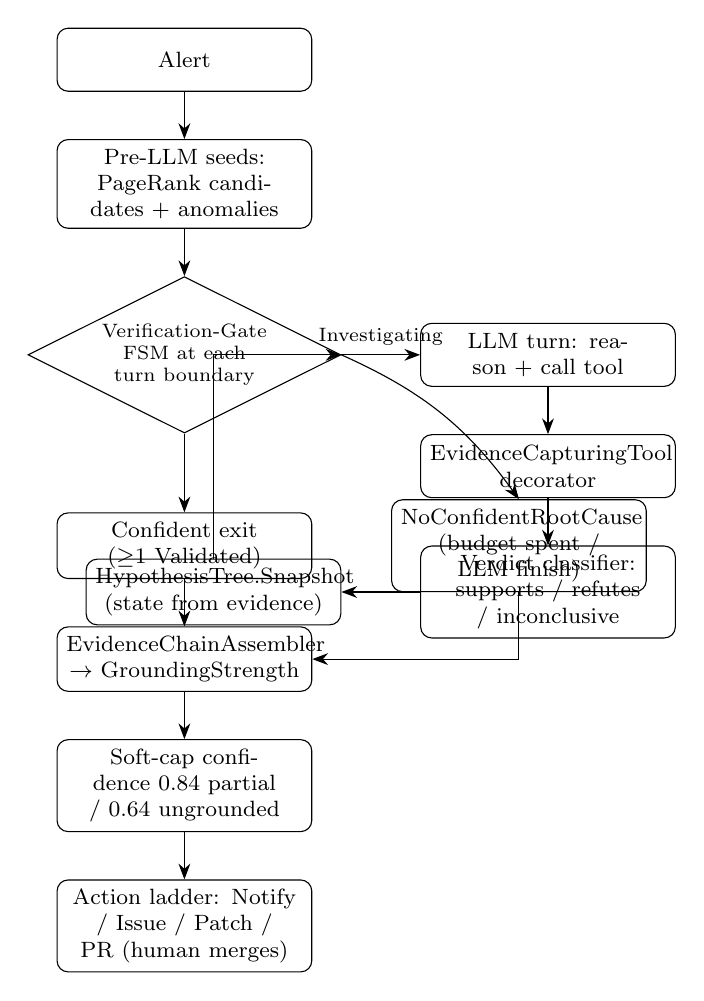
\begin{tikzpicture}[
  node distance=6mm and 10mm,
  box/.style={rectangle, draw, rounded corners, align=center,
    text width=30mm, minimum height=8mm, font=\footnotesize},
  dec/.style={diamond, draw, aspect=2, align=center,
    inner sep=1pt, font=\scriptsize, text width=22mm},
  arr/.style={-{Stealth[length=2mm]}}
]
\node[box] (alert) {Alert};
\node[box, below=of alert] (seed) {Pre-LLM seeds: PageRank candidates + anomalies};
\node[dec, below=of seed] (gate) {Verification-Gate FSM at each turn boundary};
\node[box, right=of gate] (llm) {LLM turn: reason + call tool};
\node[box, below=of llm] (cap) {EvidenceCapturingTool decorator};
\node[box, below=of cap] (verd) {Verdict classifier: supports / refutes / inconclusive};
\node[box, left=of verd] (snap) {HypothesisTree.Snapshot (state from evidence)};
\node[box, below=10mm of gate] (conf) {Confident exit ($\geq$1 Validated)};
\node[box, right=of conf] (no) {NoConfidentRootCause (budget spent / LLM finish)};
\node[box, below=of conf] (assm) {EvidenceChainAssembler $\rightarrow$ GroundingStrength};
\node[box, below=of assm] (soft) {Soft-cap confidence 0.84 partial / 0.64 ungrounded};
\node[box, below=of soft] (act) {Action ladder: Notify / Issue / Patch / PR (human merges)};

\draw[arr] (alert) -- (seed);
\draw[arr] (seed) -- (gate);
\draw[arr] (gate) -- node[above, font=\scriptsize]{Investigating} (llm);
\draw[arr] (llm) -- (cap);
\draw[arr] (cap) -- (verd);
\draw[arr] (verd) -- (snap);
\draw[arr] (snap) |- (gate);
\draw[arr] (gate) -- (conf);
\draw[arr] (gate.east) to[bend left=15] (no.north);
\draw[arr] (conf) -- (assm);
\draw[arr] (no) |- (assm);
\draw[arr] (assm) -- (soft);
\draw[arr] (soft) -- (act);
\end{tikzpicture}
\caption{The reasoning-safety core. A deterministic FSM at each turn boundary
governs exit; only a hypothesis validated by hard tool evidence yields a
``confident'' exit. Both exits flow through a pure evidence-chain assembler
and a grounding-based soft-cap before any action.}
\label{fig:core}
\end{figure}

\subsection{The externalized verification-gate FSM}

The gate is a pure, dependency-free static function ---
\texttt{VerificationGate.Evaluate} --- that the loop consults at every turn
boundary and at the voluntary-final boundary. Its file header is explicit
about lineage and intent: \emph{``a DETERMINISTIC code FSM, OUTSIDE the LLM,
that governs loop exit --- replacing MaxTurns=10 as the SOLE stop (MAST: enforce
termination via an FSM outside the model).''} It cites \texttt{FEAT-027,
FR-SG-31, NFR-SG-8, NFR-SG-2, ADR-037}.

The FSM has four states --- \texttt{Investigating},
\texttt{EvidenceSufficient}, \texttt{BudgetExhausted},
\texttt{NoConfidentRootCause} --- and emits one of three exit classifications
--- \texttt{None}, \texttt{Confident}, \texttt{NoConfidentRootCause}. The
decision precedence is fixed (no degrees of freedom):

\begin{verbatim}
public static GateDecision Evaluate(
    HypothesisTree? tree, bool llmWantsToFinish, int turnsUsed,
    TimeSpan elapsed, GateBudget budget)
{
    var validatedCount = tree?.Validated.Count ?? 0;   // fail-open: null tree => 0 (NFR-SG-2)

    if (validatedCount > 0)
        // >=1 hard-evidence hypothesis => Confident, EVEN at budget end.
        return new(GateState.EvidenceSufficient, GateExit.Confident,
                   validatedCount, tree!.RootCauseRef, false);

    if (turnsUsed >= budget.MaxTurns || elapsed >= budget.WallClock)
        // budget spent, none validated => no-confident (terminate outside the model).
        return new(GateState.BudgetExhausted, GateExit.NoConfidentRootCause, 0, null, false);

    if (llmWantsToFinish)
        // the LLM "I'm done" with nothing validated => NOT confident (core MAST guardrail).
        return new(GateState.NoConfidentRootCause, GateExit.NoConfidentRootCause, 0, null, false);

    return new(GateState.Investigating, GateExit.None, 0, null, false);
}
\end{verbatim}

Three properties matter. \textbf{(a)} A ``confident'' exit requires
\texttt{validatedCount > 0}, i.e.\ at least one hypothesis validated by hard
tool evidence; the model cannot self-terminate ``confident'' on an assertion
alone (clause 3). \textbf{(b)} Validated evidence wins \emph{even at budget
exhaustion} (clause 1 precedes clause 2): the structural budget is a stop
bound, not a suppressor of real evidence --- a \texttt{RISK-1} safety property
asserted in the change-induced eval incidents. \textbf{(c)} The gate is
\emph{fail-open and advisory} (\texttt{NFR-SG-2}): a null or empty hypothesis
tree degrades to \texttt{NoConfidentRootCause}, never throws, and never blocks
an investigation. The \texttt{AutoRemediates} field of every
\texttt{GateDecision} is hard-wired \texttt{false} (\texttt{ADR-030}) --- the
gate concludes and notifies; it never acts.

The structural budget is \texttt{GateBudget(MaxTurns, WallClock)}, in
production \texttt{MaxTurns = 10} and \texttt{WallClock = 4\,min}, nested
inside the overall 5-minute RCA run budget (\texttt{FEAT-008 FR-AG-2}). The
gate is wired into the loop through \texttt{RcaVerificationGateBinding}
against the kernel's \texttt{StopCriteria} seam, and is rolled out
\textbf{shadow-first}: in shadow mode it computes and logs its decision
without governing the loop; in active mode
(\texttt{RcaLiveActivation.Mode = active}) it governs exit. The shadow/active
flip is one of the controlled ablations in the evaluation.

\subsection{Evidence-derived hypothesis state with provenance}

The hypothesis tree is the agent's working set of candidate root causes, but
its defining property is that \emph{the LLM never sets a hypothesis's state}.
\texttt{HypothesisModel.cs} (FEAT-027 \texttt{FR-SG-28}, \texttt{FR-SG-29},
\texttt{SEC-SG-4}, \texttt{ADR-037 D1/D2}) defines a \texttt{Hypothesis} whose
\texttt{State} is \emph{computed} from its evidence list by a private
\texttt{DeriveState}:

\begin{verbatim}
private static HypothesisState DeriveState(IReadOnlyList<ToolEvidence> evidence)
{
    var hasHardSupport = false;
    var hasRefute = false;
    foreach (var e in evidence)
    {
        if (e.Verdict == EvidenceVerdict.Supports && e.IsHardToolEvidence) hasHardSupport = true;
        else if (e.Verdict == EvidenceVerdict.Refutes) hasRefute = true;
    }
    if (hasHardSupport) return HypothesisState.Validated;     // HARD tool evidence decides (D3)
    if (hasRefute)      return HypothesisState.Invalidated;   // refuted, no validating support
    return HypothesisState.Inconclusive;                      // llm-only / inconclusive / none
}
\end{verbatim}

The provenance test is a one-liner with enormous weight:

\begin{verbatim}
public bool IsHardToolEvidence => Source != EdgeSource.LlmInferred;
\end{verbatim}

A \texttt{ToolEvidence} record carries \texttt{(Tool, ResultSummary, Verdict,
Source, EvaluatedAtEpoch)}, where \texttt{Source} is an \texttt{EdgeSource}
enum drawn from the real telemetry lanes --- \texttt{Tempo}, \texttt{Loki},
\texttt{Prometheus}, \texttt{StaticInfra}, \texttt{Git}, \texttt{Synthetic}
--- \emph{or} \texttt{LlmInferred}. Only a \texttt{Supports} verdict whose
source is \emph{not} \texttt{LlmInferred} can move a hypothesis to
\texttt{Validated}. In the contract comment's words: \emph{``the model
`grading its own homework' (source = llm-inferred) is NOT hard evidence.''}
This is the structural enforcement of the MAST ``never self-verify'' rule: it
is impossible for the model to validate its own hypothesis by talking, because
validation reads only the provenance-tagged evidence list.

Evidence enters the list through the \textbf{\texttt{EvidenceCapturingTool}
decorator} (\texttt{HypothesisEvidenceCapture.cs}), which wraps every
\texttt{IAgentTool}. On each tool call it runs the raw result through a
classifier (\texttt{ToolHypothesisEvidenceClassifier}), determines which
seeded suspect the result bears on, assigns a verdict, tags the provenance
source as the real tool (never \texttt{llm-inferred}), redacts the summary to
a bounded single line ($\leq$280 chars, \texttt{SEC-SG-4} / \texttt{RISK-3}
--- never raw log lines or pod names), and records it into a
\texttt{HypothesisEvidenceSink}. The sink explicitly rejects model
self-assertion at the door:
\texttt{if (evidence.Source == EdgeSource.LlmInferred) return;}. Each
\texttt{Snapshot()} rebuilds an immutable \texttt{HypothesisTree} whose
\texttt{Conclusion} is \texttt{Validated} iff at least one hypothesis cleared
the hard-evidence bar, else the first-class \texttt{NoConfidentRootCause}.

The \textbf{verdict classifier} is \emph{negation-aware and
structured-signal-first} (\texttt{ToolEvidenceVerdict}, FEAT-027 increment-7
\texttt{FR-SG-61}). This closes a specific MAST false-positive class: a
\emph{healthy} tool result (\texttt{error\_rate: 0.00}, ``no errors'',
``0 timeouts'') must never be classified as \texttt{Supports} for a fault
hypothesis. The classifier reads structured numeric signals first and is aware
of negations in free text, so a clean health check can only ever
\texttt{Refute} or be \texttt{Inconclusive}, never falsely validate. The
first-class \texttt{NoConfidentRootCause} outcome maps, in
\texttt{RcaOutcomeMapper.Map}, into the sub-0.40 \texttt{Notify} tier --- a
\emph{deliberate} surfaced result distinct from a generic low-confidence
fallback, writing no \texttt{ROOT\_CAUSED\_BY} edge and forcing no hypothesis.

\subsection{Evidence-chain assembly and grounding-based confidence soft-cap}

The model still emits a self-rated confidence scalar in $[0,1]$. Left
unbounded, that scalar drives an action ladder --- issue at 0.40, code patches
at 0.65, an opened pull request at 0.85 --- so an over-confident,
thinly-grounded conclusion could escalate to a PR. The third mechanism
(FEAT-027 increment-5, \texttt{FR-SG-41}, \texttt{FR-SG-43},
\texttt{ADR-041}) prevents that.

At conclusion, \texttt{EvidenceChainAssembler.Assemble} runs a \textbf{pure,
no-LLM projection} over all prior signals and builds an auditable chain
comprising: the graph path to the winning suspect; the \emph{validating hard
tool evidence} (\texttt{IsHardToolEvidence \&\& Verdict == Supports} only);
the onset-window Deploy/Change \emph{citation} (the causing PR ---
\texttt{commit\_sha} or \texttt{pr\_number}, nearest-to-onset, ``no guessing''
if none); and the ranking sub-scores. From two booleans --- \emph{does a
validating hard evidence item exist?} and \emph{does a change citation exist?}
--- it derives a \texttt{GroundingStrength}:

\begin{verbatim}
private static GroundingStrength DeriveGrounding(bool hasHardEvidence, bool hasCitation) =>
    (hasHardEvidence, hasCitation) switch
    {
        (true, true)                   => GroundingStrength.Grounded,
        (true, false) or (false, true) => GroundingStrength.PartiallyGrounded,
        _                              => GroundingStrength.Ungrounded,
    };
\end{verbatim}

The \textbf{soft-cap} (\texttt{RcaEvidenceCap}) then bounds the LLM's
confidence as a function of grounding:

\begin{verbatim}
public const double CapPartial    = 0.84;   // just under the 0.85 PR tier
public const double CapUngrounded = 0.64;   // just under the 0.65 patch tier

public static double Effective(double llmConfidence, GroundingStrength g) => g switch
{
    GroundingStrength.Grounded          => llmConfidence,
    GroundingStrength.PartiallyGrounded => Math.Min(llmConfidence, CapPartial),
    GroundingStrength.Ungrounded        => Math.Min(llmConfidence, CapUngrounded),
};
\end{verbatim}

The cap is a \emph{soft} one --- it only ever lowers the score, never raises
it, and \texttt{Grounded} conclusions pass through uncapped. But the
thresholds are chosen to bite exactly at the action tiers: an
\texttt{Ungrounded} conclusion is capped at 0.64, immovably below the 0.65
patch tier, so it can never propose code; a \texttt{PartiallyGrounded} one is
capped at 0.84, immovably below the 0.85 PR tier, so it can never open a pull
request. The action-tier thresholds themselves ($0.40 / 0.65 / 0.85$) are
\emph{unchanged} across increments (\texttt{RcaOutcomeMapper},
\texttt{ADR-037 D4}); the cap operates on the input to the ladder, not the
ladder. Like the gate, the cap rolls out shadow-first and is an evaluation
ablation.

\begin{table}[ht]
\centering
\caption{Grounding-derived soft-cap. The cap operates on the input to the
action ladder; the action-tier thresholds are unchanged.}
\label{tab:cap}
\begin{tabular}{lll}
\toprule
Grounding & Condition & Effective confidence \\
\midrule
\texttt{Grounded}          & hard evidence \emph{and} citation & passes through (uncapped) \\
\texttt{PartiallyGrounded} & exactly one of the two            & $\min(\textrm{conf}, 0.84)$ --- blocks PR tier \\
\texttt{Ungrounded}        & neither                           & $\min(\textrm{conf}, 0.64)$ --- blocks patch tier \\
\bottomrule
\end{tabular}
\end{table}

Together the three mechanisms enforce a single invariant: \emph{the agent
escalates only as far as its grounding warrants, and the model's word is never
the grounding.}

\section{Implementation}

The agent is a .NET 10 FastEndpoints service. The reasoning-safety types
described above are pure and dependency-free --- \texttt{VerificationGate},
\texttt{HypothesisModel}, \texttt{EvidenceChainAssembler}, and
\texttt{RcaEvidenceCap} have no I/O --- which makes them exhaustively
unit-testable and keeps the MAST guardrails out of the model's reach by
construction. They are governed by \textbf{FEAT-027} and specifically by
\texttt{FR-SG-28} / \texttt{FR-SG-29} (hypothesis tree + first-class ``no
confident root cause''), \texttt{FR-SG-31} (externalized verification-gate
FSM), \texttt{FR-SG-41} / \texttt{FR-SG-43} (evidence chain + confidence
derivation), \texttt{FR-SG-61} (negation-aware verdict classifier),
\texttt{NFR-SG-8} (gate latency budget), \texttt{SEC-SG-7} (the PHI-egress
guard that redacts every prompt and tool result before model egress), and the
design ADRs \texttt{ADR-037} and \texttt{ADR-041}.

\paragraph{Graph and vector substrate.}
The hypothesis tree is persisted to a \texttt{bluerobin\_stack} graph in
FalkorDB (Redis wire protocol) as \texttt{Hypothesis} nodes with
\texttt{EVIDENCED\_BY} edges carrying the tool, verdict, and one-line summary;
a validated hypothesis writes the single \texttt{ROOT\_CAUSED\_BY} edge. When
graph context is serialized into the model frame, BlueRobin follows the
template triple-to-natural-language pattern that outperforms raw triples
\citep{simpleiseffective2024}. Code
retrieval and incident-memory recall use Qdrant via gRPC; embeddings are
produced locally by in-cluster Ollama, so embedding traffic never transits the
paid edge. The stack-graph also seeds the loop before any model call --- a
personalized-PageRank blame-propagation pass over the error-weighted runtime
dependency graph proposes ranked candidates, which become the \emph{seeds} the
hypothesis tree is built around (the subject of the second paper in this
series).

\paragraph{Model egress and cost.}
All LLM calls go through a single Cloudflare AI Gateway (OpenAI-compatible,
BYOK), which meters per-service spend and fails over on 402/429; a CI
guardrail (\texttt{egress-guardrail.yml}) forbids direct provider FQDNs so
egress stays Cloudflare-only. The cost angle is the headline systems claim:
the entire stack --- graph world-model, the three reasoning-safety mechanisms,
temporal incident memory, and the eval harness --- runs within a
\textbf{$\sim$50~EUR/month} platform ceiling, of which the \textbf{LLM budget
is a hard 20~EUR/month} (\texttt{COST-7}). A single Hetzner CX43
($\sim$17.5~EUR/month), Cloudflare's free tiers (R2, Tunnel, WAF), and local
Ollama embeddings carry the rest. At 100\% of the LLM budget the agent
fail-closes rather than overspend. There is no GPU, no managed RCA service,
and --- deliberately --- no causal-discovery dependency (PC/FCI/Granger are
rejected on both cost and accuracy grounds), so the reasoning-safety machinery
is the \emph{only} moving part standing between an alert and an over-confident
PR.

\paragraph{Telemetry.}
The gate emits an \texttt{OBS-SG-4} gate-outcome metric
(\texttt{confident} / \texttt{no\_confident}) and a verification-gate span per
evaluation; token usage is metered per turn into
\texttt{debug\_agent.llm\_tokens\_total\{role,model\}} and priced into a
per-RCA euro cost, so the budget constraint is observable, not merely
aspirational.

\section{Evaluation}

The agent ships with a deterministic .NET eval harness
(\texttt{RcaEvalHarness}) that replays a labelled ground-truth incident set
through the \emph{real} RCA path and emits an AC@1 (accuracy-at-1, top-1
localization) and MTTR scorecard. \textbf{We state the limitations of this
benchmark before its results, because they are severe and the authors
themselves flag the set as an ``oversimplified benchmark.''}

The dataset is \textbf{9 self-seeded labelled incidents}
(\texttt{ground-truth-incidents.json}), drawn from the existing
synthetic-test family and past replayed incidents --- \emph{not} injected with
ChaosMesh --- spanning three fault classes (auth/login, data/datastore,
deploy/config). Two are change-induced (a bad deploy to \texttt{archives-api},
a bad commit to \texttt{bluerobin-web}). AC@1 is an exact-string oracle: the
produced top-1 candidate natural key versus the labelled expected root cause.
MTTR here is a \textbf{replay-clock proxy} --- the wall-clock from
onset-replay-start to the pipeline returning its conclusion --- measured in
\emph{sub-second} values, and is explicitly \emph{not} production MTTR.

The harness has two arms. The \emph{scorer-only} arm plants the labelled cause
as an unambiguous top-1, so AC@1 = 1.0 by construction --- it is a
\textbf{regression sentinel, not an accuracy measurement}. The
\emph{live-path} arm (\texttt{ReplayLivePathAsync}) injects distractor
candidates (higher topology criticality, lower error rate --- a deliberate
topology trap) so that AC@1 $<$ 1.0 is \emph{achievable}; this is the honest
production-path arm.

\begin{table}[ht]
\centering
\caption{Eval harness arms. AC@1 = 1.0 on this 9-incident set indicates
no-regression on a benchmark too easy to discriminate the mechanisms, not a
real-world accuracy claim. MTTR is a sub-second replay-clock proxy.}
\label{tab:arms}
\begin{tabular}{p{3.2cm}p{3.0cm}ccp{3.2cm}}
\toprule
Arm & What it measures & AC@1 & MTTR (replay proxy) & Notes \\
\midrule
Scorer-only (\texttt{scorecard-baseline.json}) & Regression sentinel & 1.0 (by construction) & $\sim$0.0017\,s agg. & Not an accuracy figure \\
Live-path (\texttt{scorecard-live-path-baseline.json}) & Honest production-path localization & 1.0 (all 9, w/ distractors) & $\sim$0.0032\,s agg. & Distractors injected; AC@1 $<$ 1.0 achievable but not observed \\
Per-commit regression gate & No-regression tolerance & drop $\leq$ 0.02 & increase $\leq$ 30\,s & Fails any candidate below AC@1 0.98 or $+$30\,s MTTR \\
\bottomrule
\end{tabular}
\end{table}

The reasoning-safety mechanisms are evaluated as \textbf{shadow-vs-active
ablations}, each proving \emph{no regression} against the committed baseline
when the mechanism is activated, and \emph{byte-for-byte collapse} to baseline
when it is shadowed (the ``feature off'' control):

\begin{table}[ht]
\centering
\caption{Shadow-vs-active ablations. Each mechanism proves no AC@1 regression
when active and collapses to baseline when shadowed.}
\label{tab:ablations}
\begin{tabular}{p{3.4cm}p{3.6cm}p{3.0cm}p{4.0cm}}
\toprule
Ablation & Mechanism flipped & Flag & Result \\
\midrule
Verification gate + BARO & \texttt{VerificationGate} governs exit & \texttt{RcaLiveActivation.Mode} & No AC@1 regression; onset true-positives (GT-03, GT-07) preserved \\
Confidence soft-cap & \texttt{RcaEvidenceCap} bounds confidence & \texttt{RcaEvidenceCap.Mode} & No AC@1 regression; shadow collapses to baseline \\
Incident-memory recall & Recall fed into the LLM frame & \texttt{RcaMemory.Mode} & No AC@1 regression; shadow collapses to baseline \\
\bottomrule
\end{tabular}
\end{table}

The honest reading: on this 9-incident set the localization arm is saturated
at AC@1 = 1.0, which tells us only that the ranking path and the
reasoning-safety overlay \emph{do not regress} a benchmark that is too easy to
discriminate them. The benchmark's value is as a \textbf{per-commit safety
net} --- it provably prevents a change from silently degrading localization or
from suppressing a known change-induced true positive --- not as a measure of
real-world accuracy. The verification gate and confidence cap are, properly
speaking, \emph{not measured by AC@1 at all}: their function is to bound
over-confidence and termination behavior, which AC@1 does not score. Their
correctness is established by exhaustive unit assertions over the pure FSM and
cap functions (e.g.\ ``a clean \texttt{error\_rate: 0.00} result can never
validate a hypothesis''; ``an ungrounded conclusion is capped below 0.65''),
not by a localization number.

\section{Limitations \& Threats to Validity}

We are deliberately explicit here.

\begin{itemize}
  \item \textbf{The benchmark is oversimplified and self-seeded.} Nine
  labelled incidents, hand-seeded from existing faults, with the labelled
  cause planted as a strong top-1 (scorer arm) or top-1 among injected
  distractors (live arm). AC@1 = 1.0 is \emph{not} a real-world accuracy
  claim; it is a saturated regression sentinel. This matches the broader
  critique that current RCA benchmarks overstate capability
  \citep{rethinking2025rca}.
  \item \textbf{MTTR figures are replay-clock proxies, sub-second, and not
  production MTTR.} They measure pipeline compute latency on a seeded graph,
  not human-observed time-to-recovery. Real lifecycle KPIs (MTTD/MTTA/MTTR
  p50/p95) are computed from live incident data by a separate endpoint, but no
  production values are committed in the repository, and the corresponding SLO
  targets are deliberately left unset pending real data.
  \item \textbf{The reasoning-safety mechanisms are not scored by the
  localization benchmark.} The verification gate, the evidence-provenance
  rule, and the confidence cap are validated by unit assertions over pure
  functions, not by an end-to-end accuracy metric. We have strong evidence
  that they behave \emph{as specified}, and no large-scale evidence that they
  improve \emph{real RCA outcomes}. A proper evaluation would require a
  fault-injection corpus with confidence and termination labels, which we do
  not have.
  \item \textbf{The verdict classifier is heuristic.} The negation-aware,
  structured-signal-first classifier closes a specific MAST false-positive
  class on the tool outputs we have seen, but it is not a learned model and
  could mis-classify novel tool-output formats. Its conservatism (default to
  \texttt{Inconclusive}) is a safety bias, not a guarantee.
  \item \textbf{The system is advisory by design, and we present that as a
  strength.} A human always merges; the agent never auto-remediates
  (\texttt{AutoRemediates} is hard-\texttt{false}). Given autonomous ceilings
  of $\sim$11\% \citep[OpenRCA;][]{xu2025openrca} and $\sim$47\%
  \citep[ITBench-AA;][]{itbenchaa2026}, this is the state of the art rather
  than a compromise --- but it does mean the contributions here are about
  \emph{making the human's decision well-grounded and auditable}, not about
  autonomy.
  \item \textbf{Scale.} This is a homelab platform of roughly a dozen
  services. The mechanisms are designed to be substrate-agnostic, but we have
  not validated them on a large microservice estate, and the
  personalized-PageRank seeding that feeds the hypothesis tree is
  small-graph-friendly.
\end{itemize}

\section{Conclusion}

The failure modes that wreck LLM RCA agents are not subtle --- incorrect
self-verification, premature termination, ungrounded over-confidence --- and
they have been catalogued \citep{cemri2025mast} and re-confirmed in cautionary
studies \citep{anon2026cautionary}. The BlueRobin Debug Agent's response is to
take those modes off the table \emph{deterministically and outside the model}:
an externalized verification-gate FSM that makes ``confident'' conditional on
hard tool evidence and makes ``no confident root cause'' first-class;
hypothesis state derived purely from provenance-tagged real-tool evidence,
with the model structurally barred from grading its own homework; and a
grounding-based soft-cap that pins an ungrounded or thinly-grounded conclusion
below the action tiers that would let it propose code or open a PR. None of
this is an empirical breakthrough --- the localization benchmark is admittedly
oversimplified and the system is advisory by design --- but it is a coherent,
auditable, and \emph{reproducible} engineering discipline for building a
reasoning-safe RCA agent, and it runs in its entirety inside a
$\sim$50~EUR/month homelab budget. The contribution is the architecture and
the discipline: in agentic RCA, the safe move is to assume the model will,
given the chance, grade its own homework --- and to build the grader somewhere
it can't reach.

\bibliographystyle{plainnat}
\bibliography{references}

\end{document}
